\documentclass{article}
\usepackage[utf8]{vntex}
\usepackage{amsmath}
\usepackage{amsopn}
\usepackage{tikz}
\usetikzlibrary{matrix}

\title{Linear Algebra}
\author{Vinh Vũ}
\date{11.17.2025}

\begin{document}
\section{Matrics - Ma Trận}
\subsection{Determinant - Định Thức}

\subsubsection{Hoán Vị}
Cho ma trận
$A = \begin{pmatrix}
  1 & 2 & 3\\
  4 & 5 & 6\\
  7 & 8 & 9
\end{pmatrix}$
. Hoán vị ma trận A tức là sắp xếp các phần tử của ma trận A theo thức tự khác nhau.
$$
\begin{pmatrix}
  1 & 2 & 3\\
  4 & 5 & 6\\
  7 & 8 & 9
\end{pmatrix}\rightarrow
\begin{pmatrix}
  2 & 3 & 1\\
  7 & 9 & 8\\
  6 & 5 & 4
\end{pmatrix}
$$

\subsubsection{Nghịch Thế}
Là số cặp số mà ở đó số trước lớn hơn số sau. Ký hiệu là N.
\\Từ dãy số$A=\{3,4,5,2,1\}$. Ta có các cặp số nghịch thế sau:
\\(3,2); (3,1); (4,2); (4,2); (5,2); (5,2); (2,1)
\\$\Rightarrow N = 7$

\subsubsection{Ma Trận Vuông Cấp n}
Giả sử ma trận A là ma trận vuông cấp 2.
$$
|A| = 
\begin{vmatrix}
  a & b \\
  c & d
\end{vmatrix} = ad - bc
$$
Giả sử ma trận B là ma trận vuông cấp 3
$$
|B| = 
\begin{vmatrix}
  a & b & c\\
  d & e & f\\
  g & h & i
\end{vmatrix}
$$
Theo công thức đồ thị sau:
$$ 
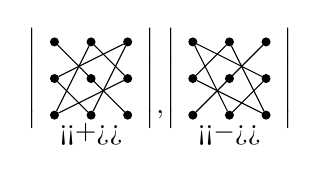
\begin{tikzpicture}
\matrix[matrix of nodes,left delimiter=|,right delimiter=|,
  row sep=1em,column sep=1em,
  nodes={draw,fill,circle,inner sep=1pt},nodes in empty cells] (m) at (0,0) {
    & & \\
    & & \\
    & & \\
  };
  \draw (m-2-1) -- (m-3-2);
  \draw (m-1-1) -- (m-3-3);
  \draw (m-1-2) -- (m-2-3);
  %
  \draw (m-1-2) -- (m-3-1);
  \draw (m-1-3) -- (m-3-2);
  %
  \draw (m-2-1) -- (m-1-3);
  \draw (m-3-1) -- (m-2-3);

  \matrix[matrix of nodes,left delimiter=|,right delimiter=|,
  row sep=1em,column sep=1em,
  nodes={draw,fill,circle,inner sep=1pt},nodes in empty cells] (n) at (5em,0) {
    & & \\
    & & \\
    & & \\
  };
  \draw (n-2-3) -- (n-3-2);
  \draw (n-1-3) -- (n-3-1);
  \draw (n-1-2) -- (n-2-1);
  %
  \draw (n-1-2) -- (n-3-3);
  \draw (n-1-1) -- (n-3-2);
  %
  \draw (n-2-3) -- (n-1-1);
  \draw (n-3-3) -- (n-2-1);

  \node at (0.0em,-2em) {<<$+$>>};
  \node at (2.5em,0 |- m.base) {$,$};
  \node at (5.0em,-2em) {<<$-$>>};
\end{tikzpicture}
$$
Ta có $|B| = aei + bfg + cdh - ceg - bdi - afh$
\\Có thể bấm máy tính để tính nhanh với những ma trận có cấp $n\geq4$.
\subsubsection{Định Thức Con và Phần Bù Đại Số}
Định thức con $|M_{ij}|$ là định thức thu được bằng cách bỏ đi hàng i và cột j của ma trận. Sau đó sử dụng phương pháp phần bù đại số để tính định thức |A|.
\\Giả sử cho ma trận A như sau:
$$
\begin{pmatrix}
  4 & 5 & 0 & 0 & 1\\
  3 & 0 & 0 & 0 & 0\\
  5 & 1 & 2 & 0 & 1\\
  2 & 6 & 0 & -1 & 1\\
  -6 & 3 & 1 & 0 & 1\\
\end{pmatrix}
\begin{pmatrix}
  + & - & + & - & +\\
  - & + & - & + & -\\
  + & - & + & - & +\\
  - & + & - & + & -\\
  + & - & + & - & +\\
\end{pmatrix}
$$
Để thực hiện phương pháp phần bù đại số, ta có chọn triển khai theo hàng hoặc cột bất kỳ, nhưng tối ưu nhất là triển khai ở nơi có chứa nhiều số 0 nhất.
\\Từ ma trận trên, ta chọn hàng 2 hoặc/và cột 4. Mục tiêu là đưa về định thức cấp 3
\begin{description}
  \item[Bước 1] Xác định hàng 2 và cột 4.
  \item[Bước 2] Chọn 1 số ở mỗi hàng và cột. VD: (-)3 ở hàng 2 và (+)-1 ở cột 4.
  \item[Bước 3] Loại bỏ hàng và cột đi qua 3 (hàng 2, cột 1) và -1(hàng 4, cột 4).
\end{description}
Từ 3 bước trên ta tính được định thức của A:
$$
|A|= (-1)\times(-3)\times
\begin{vmatrix}
  5 & 0 & 1\\
  1 & 2 & 1\\
  3 & 1 & 1
\end{vmatrix}
= 3\times(10+1-6-5)=0
$$
\subsubsection{Tính Chất Định Thức}

\begin{description}
  \item[TC1] $|AB| = |A| \times |B|$
  \item[TC2] $|A^{T}| = |A|$
  \item[TC3] Nếu đổi chỗ 2 hàng hoặc 2 cột thì định thức đổi dấu
  $$
  \begin{vmatrix}
    a & b & c\\
    d & e & f\\
    g & h & i
  \end{vmatrix}=-
  \begin{vmatrix}
    d & e & f\\
    a & b & c\\
    g & h & i
  \end{vmatrix}=-
  \begin{vmatrix}
    c & b & a\\
    f & e & d\\
    i & h & g
  \end{vmatrix}
  $$
  \item[TC4] Nếu định thức có 1 hàng/cột = 0 => định thức = 0.
  $$
  \begin{vmatrix}
    a & b & c\\
    d & e & f\\
    0 & 0 & 0
  \end{vmatrix}=0
  $$
  \item[TC5] Nếu định thức có 2 hàng/cột tỉ lệ thì định thức = 0
  $$
  \begin{vmatrix}
    a & b & c\\
    d & e & f\\
    3a & 3b & 3c
  \end{vmatrix}=0
  $$
  \item[TC6] Nếu nhân 1 hàng với K khác 0 thì định thức mới gấp K lần định thức cũ.
  \subitem Nếu A là ma trận vuông cấp n $\Rightarrow |KA| = K^{n}\times |A|$
  \subitem Rút nhân tử chung của 1 hàng/cột ra ngoài định thức.
  $$
  \begin{vmatrix}
    3 & 2 & 1\\
    6 & 4 & 1\\
    9 & 8 & 1
  \end{vmatrix}=3 \times 2 \times
  \begin{vmatrix}
    1 & 1 & 1\\
    2 & 2 & 1\\
    9 & 4 & 1
  \end{vmatrix}
  $$
  \item[TC7] Cộng 1 hàng/cột tổ hợp tuyến tính các hàng/cột $\neq$ thì định thức không đổi
  $$
    \begin{vmatrix}
    1 & 2 & 3\\
    4 & 5 & 6\\
    5 & 7 & 9
  \end{vmatrix}=0\xrightarrow{h_{3}:=h_{3}-h_{1}-h_{2}}
  \begin{vmatrix}
    1 & 2 & 3\\
    4 & 5 & 6\\
    0 & 0 & 0
  \end{vmatrix}=0
  $$
  \item[TC8] Tách định thức
   $$
  \begin{vmatrix}
    5 & 7 & 9\\
    4 & 5 & 6\\
    1 & 2 & 3
  \end{vmatrix}=
  \begin{vmatrix}
    3 & 4 & 5\\
    4 & 5 & 6\\
    1 & 2 & 3
  \end{vmatrix}+
  \begin{vmatrix}
    2 & 3 & 4\\
    4 & 5 & 6\\
    1 & 2 & 3
  \end{vmatrix}
  $$
\end{description}
\subsubsection{Phép Biến Đổi Sơ Cấp}
Tính định thức bằng phép biến đổi sơ cấp (BDSC):
\begin{itemize}
  \item Đổi chỗ 2 hàng/cột.
  \item Nhân 1 hàng/cột với $K\neq0$.
  \item Cộng vào 1 hàng/cột tổ hợp tuyến tính hàng/cột $\neq$
\end{itemize}
Mục tiêu: Đưa định thức về định thức tam giác (có nhiều số 0)
$$
\begin{vmatrix}
  1 & -3 & 2 & 7\\
  1 & -2 & 1 & 6\\
  3 & -9 & 7 & 2\\
  2 & 5 & -2 & -2
\end{vmatrix}\xrightarrow[h_{3}:=h_{3}-3h_{1} | h_{4}:=h_{4}-2h_{1}]{h_{2}:=h_{2}-h{1}}
\begin{vmatrix}
  1 & -3 & 2 & 7\\
  0 & 1 & -1 & -1\\
  0 & 0 & 1 & -19\\
  0 & 11 & -5 & -16
\end{vmatrix}
$$
$$
\xrightarrow{h_{4}:=h_{4}-11h_{2}}
\begin{vmatrix}
  1 & -3 & 2 & 7\\
  0 & 1 & -1 & -1\\
  0 & 0 & 1 & -19\\
  0 & 0 & 6 & -5
\end{vmatrix}\xrightarrow{h_{4}:=h_{4}-6h_{3}}
\begin{vmatrix}
  1 & -3 & 2 & 7\\
  0 & 1 & -1 & -1\\
  0 & 0 & 1 & -19\\
  0 & 0 & 0 & 109
\end{vmatrix}
$$
$$
\Rightarrow |A| =1 \times 1 \times 1 \times 109 = 109
$$

\end{document}